    \subsection*{Initialization}
    
        The first problem we have is related to something we mentioned at the end of the last section: $k$-means is not \textbf{convex}. 
        
        That means we can find \textbf{local} minima that are not the \textbf{global} minimum: our \textbf{initialization} (our \textbf{starting} clusters) can affect whether we end up in a useful minimum.
            \note{The reason why is, mathematically, the same as when we first introduced the idea of a local minimum.}
            
        \begin{figure}[H]
            \centering
            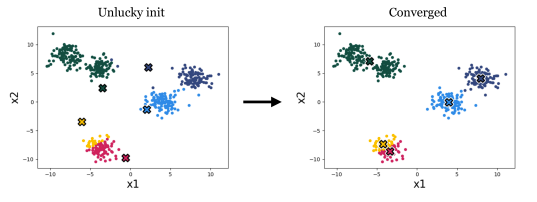
\includegraphics[width=100mm,scale=0.4]{images/clustering_images/unlucky_init.png}
            \caption*{In this example, notice that we ended up with convergence on some very \textbf{bad} clusters: the bottom cluster is split in \textbf{half}!}
        \end{figure}
        
        The easiest way to resolve this is to run $k$-means multiple times with different initializations.
            \note{Other techniques exist, but this is the simplest one.}\\
        
        \begin{concept}
            Getting an \vocab{unlucky initialization} can result in \purp{clusters} that aren't \gren{useful}.
            
            We try to \gren{solve} this by running our algorithm \purp{multiple times}.
        \end{concept}